\chapter{Resoconto attività di verifica } \label{ResocontoAttivitàDiVerifica}
In questa sezione si riportano gli esiti, descritti ed analizzati, di tutte le attività$_{\scaleto{G}{3pt}}$ di verifica svolte.
\section{Revisione dei Requisiti}  \label{ResocontoAttivitàDiVerificaRevisioneDeiRequisiti}
Tutta la documentazione sviluppata nella prima fase da consegnare per la Revisione dei Requisiti ha subito una meticolosa ed attenta revisione da parte dei Verificatori. Questi ultimi hanno seguito, in questa attività$_{\scaleto{G}{3pt}}$, per ogni documento, i metodi di \textit{Walkthrough$_G$} ed \textit{Inspection$_G$} relative all’analisi statica, stabilite nelle \textit{Norme di Progetto 3.0.0}.
\subsection{Strategia adoperata per l’analisi statica dei documenti} \label{ResocontoAttivitàDiVerificaRevisioneDeiRequisitiStrategiaPerAnalisiStatica}
Il \textit{Verificatore} si è occupato di valutare la correttezza del documento, concentrandosi nell’individuare gli errori presenti in questo. Una volta individuati gli errori la strategia adottata è la seguente:
\begin{itemize}
	\item Correzione degli errori sia ortografici che sintattici, non fedeli alle norme tipografiche fissate nelle \textit{Norme di Progetto 3.0.0}.
\end{itemize}

\subsection{Esiti verifica} \label{ResocontoAttivitàDiVerificaRevisioneDeiRequisitiEsitiVerifica}
Per ciascun documento stilato si è calcolato l’indice di Gulpease$_{\scaleto{G}{3pt}}$. I risultati sono mostrati qui di seguito.
Per evitare risultati errati nel calcolo di tale indice, non si sono tenuti in considerazione:
\begin{itemize}
	\item il frontespizio di ogni documento;
	\item le eventuali tabelle presenti nel documenti;
	\item i diari delle modifiche di ogni documento.
\end{itemize}

\quad
\def\tabularxcolumn#1{m{#1}}
{\rowcolors{2}{RawSienna!90!RawSienna!20}{RawSienna!70!RawSienna!40}
	\begin{center}
		\renewcommand{\arraystretch}{1.4}
		\begin{tabularx}{11.50cm}{|c|c|c|}
			\hline
			\rowcolor{airforceblue}
			\textbf{Documento} & \textbf{Indice di Gulpease} & \textbf{Esito}\\
			\hline
			\textit{Analisi dei Requisiti 1.0.0} & 96  & \textit{Superato}\\
			\hline
			\textit{Norme di Progetto 1.0.0} & 75 & \textit{Superato}\\
			\hline
			\textit{Studio di Fattibilità 1.0.0} & 70 & \textit{Superato}\\
			\hline
			\textit{Piano di Progetto 1.0.0} & 77 & \textit{Superato}\\
			\hline
			\textit{Piano di Qualifica 1.0.0} & 80 & \textit{Superato}\\
			\hline
		\end{tabularx}
		\captionof{table}{\textbf{Elenco Indici di Gulpease$_{\scaleto{G}{3pt}}$ dei documenti fino alla RR}}
	\end{center}


\begin{figure}[!h]
	\begin{center}
		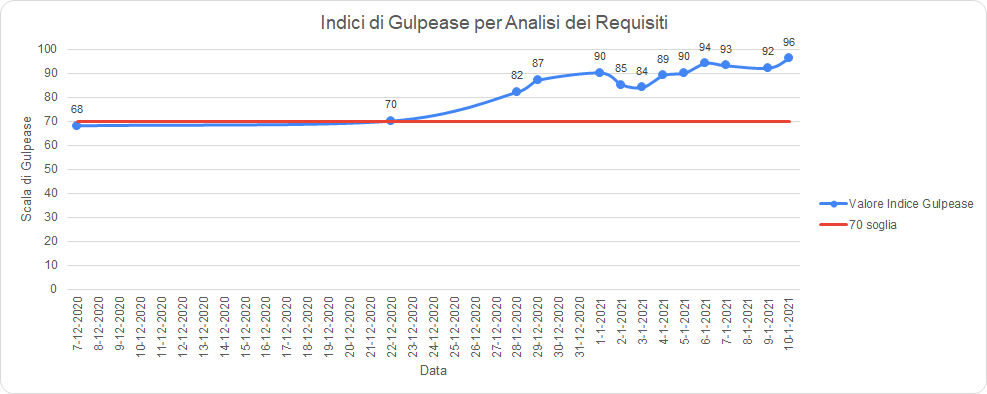
\includegraphics[width=1\linewidth]{../immagini/IndexGulpeaseAdR.png}
		\caption{\textbf{Andamento Indice di Gulpease$_{\scaleto{G}{3pt}}$ Analisi dei Requisiti fino a RR}}
	\end{center}
\end{figure}

\begin{figure}[!h]
	\begin{center}
		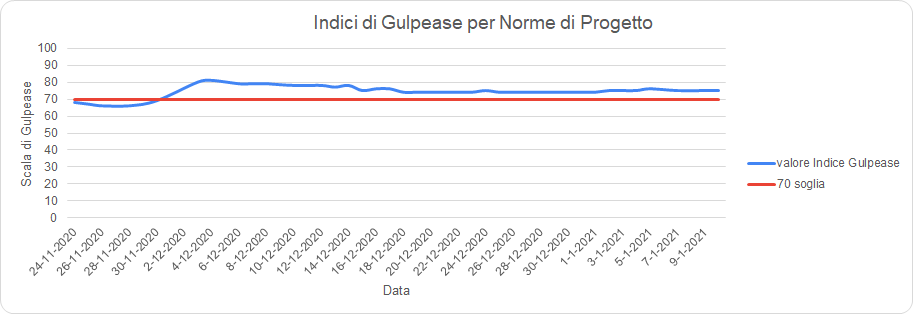
\includegraphics[width=1\linewidth]{../immagini/IndexGulpeaseNdP.png}
		\caption{\textbf{Andamento Indice di Gulpease$_{\scaleto{G}{3pt}}$ Norme di Progetto fino a RR}}
	\end{center}
\end{figure}

\begin{figure}[!h]
	\begin{center}
		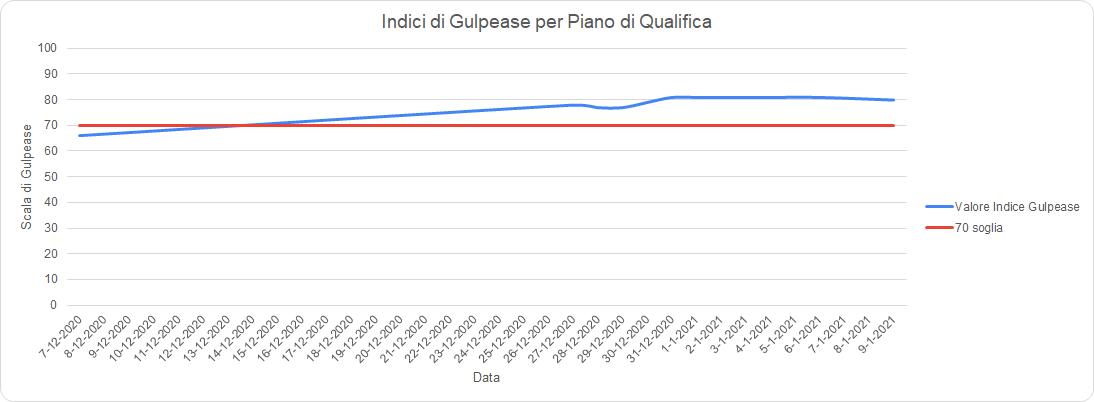
\includegraphics[width=1\linewidth]{../immagini/IndexGulpeasePdQ.png}
		\caption{\textbf{Andamento Indice di Gulpease$_{\scaleto{G}{3pt}}$ Piano di Qualifica fino a RR}}
	\end{center}
\end{figure}

\begin{figure}[!h]
	\begin{center}
		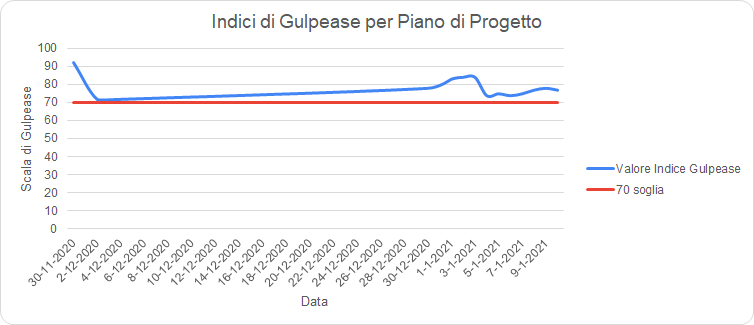
\includegraphics[width=1\linewidth]{../immagini/IndexGulpeasePdP.png}
		\caption{\textbf{Andamento Indice di Gulpease$_{\scaleto{G}{3pt}}$ Piano di Progetto fino a RR}}
	\end{center}
\end{figure}

\begin{figure}[H]
	\begin{center}
		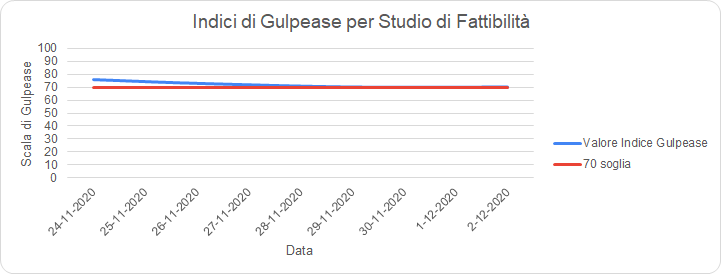
\includegraphics[width=1\linewidth]{../immagini/IndexGulpeaseSdF.png}
		\caption{\textbf{Andamento Indice di Gulpease$_{\scaleto{G}{3pt}}$ Studio di Fattibilità fino a RR}}
	\end{center}
\end{figure}

Per quanto riguarda gli Indici di Gulpease$_{\scaleto{G}{3pt}}$ dei verbali si è deciso di rappresentare i risultati in forma tabellare.
Questo in quanto il verbale viene scritto tutta in una volta, quindi utilizzare un grafico temporale risulta non idoneo.
\quad
\def\tabularxcolumn#1{m{#1}}
{\rowcolors{2}{RawSienna!90!RawSienna!20}{RawSienna!70!RawSienna!40}
	\begin{center}
		\renewcommand{\arraystretch}{1.4}
		\begin{tabularx}{11.65cm}{|c|c|c|}
			\hline
			\rowcolor{airforceblue}
			\textbf{Documento} & \textbf{Indice di Gulpease} & \textbf{Esito}\\
			\hline
			\textit{verbale\_interno\_2020-10-28} & 100  & \textit{Superato}\\
			\hline
			\textit{verbale\_interno\_2020-11-19} & 100 & \textit{Superato}\\
			\hline
			\textit{verbale\_interno\_2020-11-24} & 99 & \textit{Superato}\\
			\hline
			\textit{verbale\_interno\_2020-12-04} & 98 & \textit{Superato}\\
			\hline
			\textit{verbale\_esterno\_2020-12-17} & 99 & \textit{Superato}\\
			\hline
			\textit{verbale\_interno\_2020-12-29} & 100 & \textit{Superato}\\
			\hline
			\textit{verbale\_interno\_2021-01-03} & 100 & \textit{Superato}\\
			\hline
			\textit{verbale\_interno\_2021-01-06} & 100 & \textit{Superato}\\
			\hline
		\end{tabularx}
		\captionof{table}{\textbf{Elenco Indici di Gulpease$_{\scaleto{G}{3pt}}$ dei verbali fino alla RR}}
	\end{center}

\section{Revisione di Progettazione} \label{ResocontoAttivitàDiVerificaRevisioneDiProgettazione}
Tutta la documentazione da consegnare per la Revisione dei Progettazione ha subito una meticolosa ed attenta revisione da parte dei Vericatori. Questi ultimi
hanno seguito, per ogni documento, i metodi di \textit{Walkthrough$_G$} ed \textit{Inspection$_G$} relativi all'analisi statica, stabiliti nelle \textit{Norme di Progetto 2.0.0}.

\subsection{Verifiche di processo} \label{RevisioneDiProgettazioneVerificheDiProcesso}
\begin{center}
 \begin{figure}[H]
	 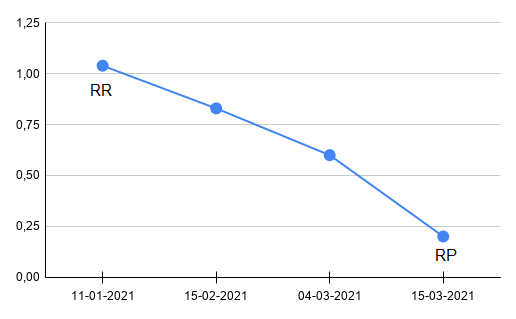
\includegraphics[width=1\linewidth]{../immagini/Metriche/MQPS05.png}
	 \caption{\textbf{MQPS05}}
 \end{figure}
\end{center}

Il grafico indica la variazione di giorni di lavoro, dove l'asse dello zero individua il rispetto dei tempi di lavoro. Da questo si evidenzia come in entrambe le fasi ci sia una maggiorazione di giorni di lavoro rispetto a quelli preventivati. Anche se presente una maggiorazione si può notare come il gruppo sia riuscito ad ottimizzare il lavoro dalla \textit{Revisione dei Requisiti} per diminuire il più possibile questo difetto.
 \subsection{Verifiche di prodotto} \label{ResocontoAttivitàDiVerificaRevisioneDiProgettazioneVerificheDiProdotto}
\subsubsection{Strategia adoperata per l’analisi statica dei documenti} \label{ResocontoAttivitàDiVerificaRevisioneDiProgettazioneVerificheDiProdottoStrategiaPerAnalisiStatica}
La strategia adoperata per l’analisi statica dei documenti per la \textit{Revisione di Progettazione} è la medesima di quella descritta in \S~\ref{ResocontoAttivitàDiVerificaRevisioneDeiRequisitiStrategiaPerAnalisiStatica}.
\paragraph{Esiti Verifica} \label{ResocontoAttivitàDiVerificaRevisioneDiProgettazioneVerificheDiProdottoStrategiaPerAnalisiStaticaEsitiVerifica}
Per ciascun documento stilato si è calcolato l’indice di Gulpease$_{\scaleto{G}{3pt}}$. I risultati sono mostrati qui di seguito.
Per evitare risultati errati nel calcolo di tale indice, non si sono tenuti in considerazione:
\begin{itemize}
	\item il frontespizio di ogni documento;
	\item le eventuali tabelle presenti nel documenti;
	\item i diari delle modifiche di ogni documento.
\end{itemize}
\quad
\def\tabularxcolumn#1{m{#1}}
{\rowcolors{2}{RawSienna!90!RawSienna!20}{RawSienna!70!RawSienna!40}
	\begin{center}
		\renewcommand{\arraystretch}{1.4}
		\begin{tabularx}{11.50cm}{|c|c|c|}
			\hline
			\rowcolor{airforceblue}
			\textbf{Documento} & \textbf{Indice di Gulpease} & \textbf{Esito}\\
			\hline
			\textit{Analisi dei Requisiti 3.0.0} & 92  & \textit{Superato}\\
			\hline
			\textit{Norme di Progetto 2.0.0} & 86 & \textit{Superato}\\
			\hline
			\textit{Piano di Progetto 2.0.0} & 79 & \textit{Superato}\\
			\hline
			\textit{Piano di Qualifica 2.0.0} & 84 & \textit{Superato}\\
			\hline
		\end{tabularx}
		\captionof{table}{\textbf{Elenco Indici di Gulpease$_{\scaleto{G}{3pt}}$ dei documenti fino alla RP}}
	\end{center}

\begin{figure}[!h]
	\begin{center}
		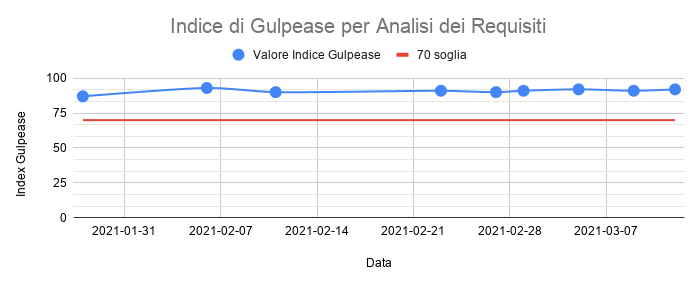
\includegraphics[width=1\linewidth]{../immagini/gulpeaseRP/IndicediGulpease perAnalisiDeiRequisiti.png}
		\caption{\textbf{Andamento Indice di Gulpease$_{\scaleto{G}{3pt}}$ Analisi dei Requisiti fino a RP}}
	\end{center}
\end{figure}

\begin{figure}[H]
	\begin{center}
		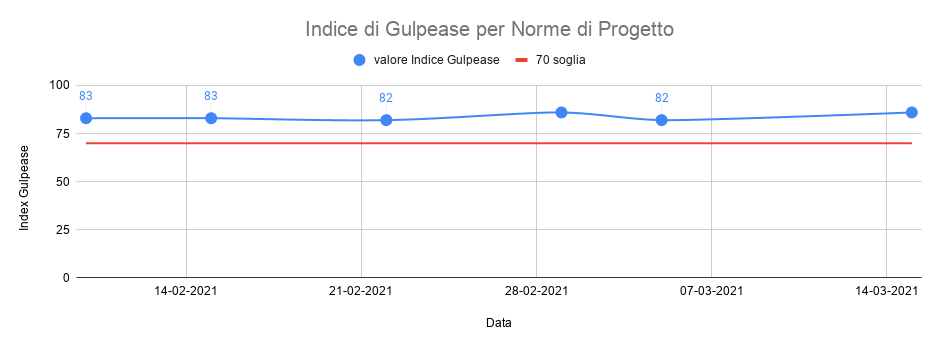
\includegraphics[width=1\linewidth]{../immagini/gulpeaseRP/IndicediGulpeaseperNormediProgetto.png}
		\caption{\textbf{Andamento Indice di Gulpease$_{\scaleto{G}{3pt}}$ Norme di Progetto fino a RP}}
	\end{center}
\end{figure}

\begin{figure}[H]
	\begin{center}
		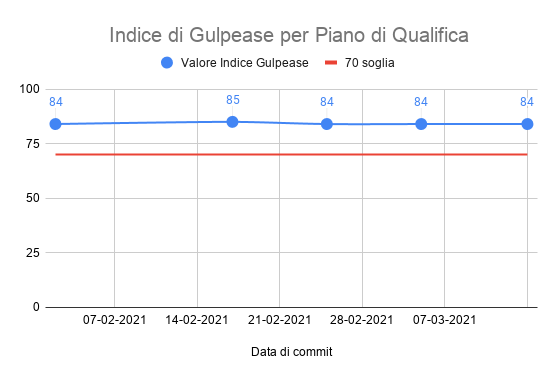
\includegraphics[width=0.9\linewidth]{../immagini/gulpeaseRP/indPdQ2.png}
		\caption{\textbf{Andamento Indice di Gulpease$_{\scaleto{G}{3pt}}$ Piano di Qualifica fino a RP}}
	\end{center}
\end{figure}

\begin{figure}[H]
	\begin{center}
		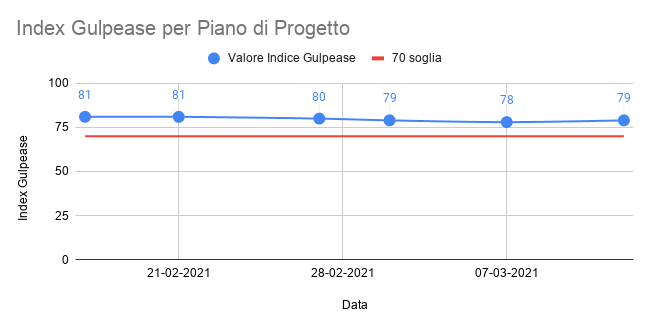
\includegraphics[width=0.9\linewidth]{../immagini/gulpeaseRP/indPdP2.png}
		\caption{\textbf{Andamento Indice di Gulpease$_{\scaleto{G}{3pt}}$ Piano di Progetto fino a RP}}
	\end{center}
\end{figure}

%ALTRI GRAFICI

Per quanto riguarda gli Indici di Gulpease$_{\scaleto{G}{3pt}}$ dei verbali si è deciso di rappresentare i risultati in forma tabellare.
Questo in quanto il verbale viene scritto tutta in una volta, quindi utilizzare un grafico temporale risulta non idoneo.

\quad
\def\tabularxcolumn#1{m{#1}}
{\rowcolors{2}{RawSienna!90!RawSienna!20}{RawSienna!70!RawSienna!40}
	\begin{center}
		\renewcommand{\arraystretch}{1.4}
		\begin{tabularx}{9.5cm}{|c|c|c|}
			\hline
			\rowcolor{airforceblue}
			\textbf{Documento} & \textbf{Indice di Gulpease} & \textbf{Esito}\\
			\hline
			\textit{v\_e\_2021-01-28} & 99 & \textit{Superato}\\
			\hline
			\textit{v\_i\_2021-01-29} & 98  & \textit{Superato}\\
			\hline
			\textit{v\_e\_2021-02-02} & 100 & \textit{Superato}\\
			\hline
			\textit{v\_e\_2021-02-08} & 100 & \textit{Superato}\\
			\hline
			\textit{v\_i\_2021-02-10} & 100 & \textit{Superato}\\
			\hline
			\textit{v\_i\_2021-02-17} & 99 & \textit{Superato}\\
			\hline
			\textit{v\_e\_2021-02-25} & 98 & \textit{Superato}\\
			\hline
			\textit{v\_i\_2021-02-26} & 100 & \textit{Superato}\\
			\hline

			\textit{v\_i\_2021-03-08} & 100 & \textit{Superato}\\
			\hline
		\end{tabularx}
		\captionof{table}{\textbf{Elenco Indici di Gulpease$_{\scaleto{G}{3pt}}$ dei verbali fino alla RP}}
	\end{center}

\section{Revisione di qualifica}\label{ResocontoAttivitàDiVerificaRevisioneDiQualifica}
Tutta la documentazione da consegnare per la Revisione di Qualifica ha subito una meticolosa ed attenta revisione da parte dei Verificatori. Questi ultimi, per attuare la verifica, hanno seguito per ogni documento i metodi di \textit{Walkthrough}$_{\scaleto{G}{3pt}}$ ed \textit{Inspection}$_{\scaleto{G}{3pt}}$, relativi all'analisi statica stabiliti nelle \textit{Norme di Progetto 3.0.0}.

\subsection{Verifiche di processo}\label{ResocontoAttivitàDiVerificaRevisioneDiQualificaVerificheDiProcesso}

\subsubsection{MQPS05}\label{ResocontoAttivitàDiVerificaRevisioneDiQualificaVerificheDiProcessoMPQS05}

Il grafico sottostante indica la variazione di giorni di lavoro dove l'asse zero individua il rispetto dei tempi di lavoro.

\subsubsection{PROI}\label{ResocontoAttivitàDiVerificaRevisioneDiQualificaVerificheDiProcessoPROI}

Il numero di requisiti$_{\scaleto{G}{3pt}}$ e la loro suddivisione in implementati e non implementati è visualizzabile nella seguente tabella.

\quad
\def\tabularxcolumn#1{m{#1}}
{\rowcolors{2}{RawSienna!90!RawSienna!20}{RawSienna!70!RawSienna!40}
	\begin{center}
		\renewcommand{\arraystretch}{1.4}
		\begin{longtable}[c]{|p{4cm}|p{3cm}|}
			\hline
			\rowcolor{airforceblue}
			\makecell[c]{\textbf{Realizzazione}} & \makecell[c]{\textbf{Quantità}}\\
			\hline
			\textit{Implementato} & \makecell[c]{45}\\
			\hline
			\textit{Non Implementato} & \makecell[c]{1} \\
			\hline
			\textit{Totali} & \makecell[c]{46} \\
		\end{longtable}
		\captionof{table}{\textbf{PROI}}
	\end{center}

Effettuando il calcolo di questa metrica otteniamo una percentuale di requisiti obbligatori implementati pari ad un valore accettabile di 98\%.

\subsection{Verifiche di prodotto}\label{ResocontoAttivitàDiVerificaRevisioneDiQualificaVerificheDiProdotto}

\subsubsection{MQPD01}\label{ResocontoAttivitàDiVerificaRevisioneDiQualificaVerificheDiProcessoMQPD01}

Il numero di requisiti$_{\scaleto{G}{3pt}}$ \textit{funzionali} e la loro suddivisione in implementati e non implementati è presente nella seguente tabella.

\quad
\def\tabularxcolumn#1{m{#1}}
{\rowcolors{2}{RawSienna!90!RawSienna!20}{RawSienna!70!RawSienna!40}
	\begin{center}
		\renewcommand{\arraystretch}{1.4}
		\begin{longtable}[c]{|p{4cm}|p{3cm}|}
			\hline
			\rowcolor{airforceblue}
			\makecell[c]{\textbf{Realizzazione}} & \makecell[c]{\textbf{Quantità}}\\
			\hline
			\textit{Implementato} & \makecell[c]{35}\\
			\hline
			\textit{Non Implementato} & \makecell[c]{22} \\
			\hline
			\textit{Totali} & \makecell[c]{57} \\
		\end{longtable}
		\captionof{table}{\textbf{MQPD01}}
	\end{center}

Effettuando il calcolo di questa metrica, otteniamo una percentuale di totalità dei requisiti \textit{funzionali} pari al 37\%, valore non accettabile, dovuto all'alto numero di requisiti funzionali non implementati in quanto non obbligatori. Per migliorare questo valore il gruppo si impegna nel cercare di implementare quanti più possibili requisiti non obbligatori nel periodo che intercorre tra la revisione di qualifica e la revisione di accettazione.

\subsubsection{MQPD03}\label{ResocontoAttivitàDiVerificaRevisioneDiQualificaVerificheDiProcessoMQPD03}

Il gruppo ha iniziato a svolgere i primi test di unità dei differenti moduli sviluppati. Di seguito è presente una tabella che indica il numero dei test eseguiti, i test che passano e i test che generano errori.\\
\textit{Nel caso in cui il gruppo riesca a trovare un'implementazione dei test di unità del modulo legato al machine learning$_{\scaleto{G}{3pt}}$, la metrica verrà aggiornata nella fase successiva}

\quad
\def\tabularxcolumn#1{m{#1}}
{\rowcolors{2}{RawSienna!90!RawSienna!20}{RawSienna!70!RawSienna!40}
	\begin{center}
		\renewcommand{\arraystretch}{1.4}
		\begin{longtable}[c]{|p{3cm}|p{3cm}|p{3cm}|p{4cm}|}
			\hline
			\rowcolor{airforceblue}
			\makecell[c]{\textbf{Modulo}} & \makecell[c]{\textbf{Test totali}} & \makecell[c]{\textbf{Test passati}} & \makecell[c]{\textbf{Test non passati}} \\
			\hline
			\textit{Acquisizione} & \makecell[c]{3} & \makecell[c]{3} & \makecell[c]{0} \\
			\hline
			\textit{Back-end} & \makecell[c]{4} & \makecell[c]{4} & \makecell[c]{0} \\
			\hline
			\textit{Front-end} & \makecell[c]{21} & \makecell[c]{18} & \makecell[c]{3}\\
			\hline
		\end{longtable}
		\captionof{table}{\textbf{Tabella dei test di unità effettuati}}
	\end{center}

Di seguito è presente una tabella che indica il valore di questa metrica per ogni modulo sviluppato ed infine il valore somma di ogni modulo. L'unico modulo ancora non testato è quello di predizione, legato al machine learning$_G$, in quanto varia ad ogni esecuzione.

\quad
\def\tabularxcolumn#1{m{#1}}
{\rowcolors{2}{RawSienna!90!RawSienna!20}{RawSienna!70!RawSienna!40}
	\begin{center}
		\renewcommand{\arraystretch}{1.4}
		\begin{longtable}[c]{|p{4cm}|p{4cm}|}
			\hline
			\rowcolor{airforceblue}
			\makecell[c]{\textbf{Modulo}} & \makecell[c]{\textbf{Valore metrica}}\\
			\hline
			\textit{Acquisizione} & \makecell[c]{0\%} \\
			\hline
			\textit{Back-end} &  \makecell[c]{14\%}\\
			\hline
			\textit{Front-end} & \makecell[c]{0\%} \\
			\hline
			\textit{Totale} & \makecell[c]{11\%}\\
			\hline
		\end{longtable}
		\captionof{table}{\textbf{MQPD03}}
	\end{center}

Il valore totale di questa metrica risulta non accettabile in quanto superiore al 10\%. Il gruppo si propone di raggiungere il valore accettabile riducendo i test con errore presenti.

\subsubsection{MQPD04}\label{ResocontoAttivitàDiVerificaRevisioneDiQualificaVerificheDiProcessoMQPD04}

Il calcolo di questa metrica non è possibile automatizzarlo in quanto è relativo al numero di persone contate dal software contapersone. Il controllo e il calcolo della metrica avvengono in intervalli di tempo periodici programmati. La media ottenuta è circa pari al 75\%.

\subsubsection{MQPD05}\label{ResocontoAttivitàDiVerificaRevisioneDiQualificaVerificheDiProcessoMQPD05}

Poiché questa metrica è legata alla comprensione del codice, il gruppo ha deciso di evidenziarla attraverso la seguente tabella dove verranno mostrati i risultati per ogni modulo di sviluppo ed infine il risultato somma di ogni modulo.

\quad
\def\tabularxcolumn#1{m{#1}}
{\rowcolors{2}{RawSienna!90!RawSienna!20}{RawSienna!70!RawSienna!40}
	\begin{center}
	\renewcommand{\arraystretch}{1.4}
	\begin{longtable}[c]{|p{4cm}|p{4cm}|}
			\hline
			\rowcolor{airforceblue}
			\makecell[c]{\textbf{Modulo}} & \makecell[c]{\textbf{Valore metrica}}\\
			\hline
			\textit{Acquisizione} & \makecell[c]{27\%} \\
			\hline
			\textit{Predizione} & \makecell[c]{18\%}\\
			\hline
			\textit{Back-end} &  \makecell[c]{11\%}\\
			\hline
			\textit{Front-end} & \makecell[c]{0,2\%} \\
			\hline
			\textit{Totale} & \makecell[c]{8\%}\\
			\hline
		\end{longtable}
		\captionof{table}{\textbf{MQPD05}}
	\end{center}

Il modulo di acquisizione presenta un valore non accettabile perché superiore al 20\%. I commenti presenti all'interno dei file di tale modulo sono necessari alla comprensione del codice riguardante l'esecuzione delle librerie esterne. L'incidenza di questo valore non rende il totale superiore alla soglia preferibile prevista.

\subsubsection{MQPD06}\label{ResocontoAttivitàDiVerificaRevisioneDiQualificaVerificheDiProcessoMQPD06}

Di seguito è presente la tabella che indica il numero di volte che ogni modulo venga utilizzato da un dato modulo.

\quad
\def\tabularxcolumn#1{m{#1}}
{\rowcolors{2}{RawSienna!90!RawSienna!20}{RawSienna!70!RawSienna!40}
	\begin{center}
		\renewcommand{\arraystretch}{1.4}
		\begin{longtable}[c]{|p{3cm}|p{5cm}|p{5cm}|}
			\hline
			\rowcolor{airforceblue}
			\makecell[c]{\textbf{Modulo}} & \makecell[c]{\textbf{Numero di chiamate}} & \makecell[c]{\textbf{Modulo chiamante}}\\
			\hline
			\textit{Acquisizione} & \makecell[c]{0} & \makecell[c]{-}\\
			\hline
			\textit{Predizione} & \makecell[c]{0} & \makecell[c]{-}\\
			\hline
			\textit{Back-end} &  \makecell[c]{1} & \makecell[c]{Front end}\\
			\hline
			\textit{Front-end} &  \makecell[c]{0} & \makecell[c]{-}\\
			\hline
			\textit{Totale} & \makecell[c]{1} & \makecell[c]{Front end}\\
			\hline
		\end{longtable}
		\captionof{table}{\textbf{MQPD06}}
	\end{center}

Il valore di questa metrica, come si può evincere dalla tabella, è pari al valore preferibile ovvero 1. Se si dovesse considerare il database come modulo, questo valore sarebbe nettamente maggiore ma il gruppo ha deciso di non includerlo nel conteggio perchè si otterrebbe un valore non veritiero dello structural fan-in.

\subsubsection{Strategia adoperata per l'analisi statica dei documenti}\label{ResocontoAttivitàDiVerificaRevisioneDiQualificaVerificheDiProdottoStrategiaAdoperataPerLAnalisiStaticaDeiDocumenti}
La strategia adoperata per l’analisi statica dei documenti per la \textit{Revisione di Progettazione} è la medesima di quella descritta in \S~\ref{ResocontoAttivitàDiVerificaRevisioneDeiRequisitiStrategiaPerAnalisiStatica}.

\paragraph{Esiti verifica}\label{ResocontoAttivitàDiVerificaRevisioneDiQualificaVerificheDiProdottoStrategiaAdoperataPerLAnalisiStaticaDeiDocumentiEsitiDiVerifica}
Per ciascun documento stilato si è calcolato l’indice di Gulpease$_{\scaleto{G}{3pt}}$. I risultati sono mostrati qui di seguito.
Per evitare risultati errati nel calcolo di tale indice, non si sono tenuti in considerazione:
\begin{itemize}
	\item il frontespizio di ogni documento;
	\item le eventuali tabelle presenti nel documenti;
	\item i diari delle modifiche di ogni documento.
\end{itemize}
\quad
\def\tabularxcolumn#1{m{#1}}
{\rowcolors{2}{RawSienna!90!RawSienna!20}{RawSienna!70!RawSienna!40}
	\begin{center}
		\renewcommand{\arraystretch}{1.4}
		\begin{tabularx}{11,70cm}{|c|c|c|}
			\hline
			\rowcolor{airforceblue}
			\textbf{Documento} & \textbf{Indice di Gulpease} & \textbf{Esito}\\
			\hline
			\textit{Analisi dei Requisiti 4.0.0} &  & \textit{Superato}\\
			\hline
			\textit{Norme di Progetto 3.0.0} & & \textit{Superato}\\
			\hline
			\textit{Piano di Progetto 3.0.0} &  & \textit{Superato}\\
			\hline
			\textit{Piano di Qualifica 3.0.0} &  & \textit{Superato}\\
			\hline
			\textit{Manuale Utente 1.0.0} & & \textit{Superato}\\
			\hline
			\textit{Manuale Sviluppatore 1.0.0} & & \textit{Superato}\\
			\hline
			\textit{Product Baseline 1.0.0} & & \textit{Superato}\\
			\hline
		\end{tabularx}
		\captionof{table}{\textbf{Elenco Indici di Gulpease$_{\scaleto{G}{3pt}}$ dei documenti fino alla RQ}}
	\end{center}

Per quanto riguarda gli Indici di Gulpease$_{\scaleto{G}{3pt}}$ dei verbali si è deciso di rappresentare i risultati in forma tabellare.
Questo in quanto il verbale viene scritto tutta in una volta, quindi utilizzare un grafico temporale risulta non idoneo.

\quad
\def\tabularxcolumn#1{m{#1}}
{\rowcolors{2}{RawSienna!90!RawSienna!20}{RawSienna!70!RawSienna!40}
	\begin{center}
		\renewcommand{\arraystretch}{1.4}
		\begin{tabularx}{9.5cm}{|c|c|c|}
			\hline
			\rowcolor{airforceblue}
			\textbf{Documento} & \textbf{Indice di Gulpease} & \textbf{Esito}\\
			\hline
			\textit{v\_e\_2021-03-19} & 98 & \textit{Superato}\\
			\textit{v\_e\_2021-03-25} & 100 & \textit{Superato}\\
			\textit{v\_i\_2021-03-26} & 99 & \textit{Superato}\\
			\textit{v\_e\_2021-03-29} & 99 & \textit{Superato}\\
			\textit{v\_e\_2021-03-31} & 100 & \textit{Superato}\\
			\textit{v\_i\_2021-04-09} & 100 & \textit{Superato}\\
			\textit{v\_i\_2021-04-12} & 100 & \textit{Superato}\\
			\textit{v\_e\_2021-04-15} & 98 & \textit{Superato}\\
			\textit{v\_e\_2021-04-16} & 99 & \textit{Superato}\\
			\textit{v\_i\_2021-04-19} & 100 & \textit{Superato}\\
			\hline
		\end{tabularx}
		\captionof{table}{\textbf{Elenco Indici di Gulpease$_{\scaleto{G}{3pt}}$ dei verbali fino alla RQ}}
	\end{center}